\section{Implementazione}

Esponiamo ora alcuni dettagli implementativi relativi alla struttura delle reti e alla loro logica evolutiva. 

%implementazione della struttura
\begin{itemize}
    \item Per quanto riguarda l'implementazione della \textit{struttura della rete neurale} per modellare l'uscita corrente dei neuroni di un layer si è deciso di ricorrere a dei dizionari: la chiave rappresenta l'id del neurone e l'elemento relativo è il valore di uscita corrente del neurone.
    I vari dizionari che rappresentano i layer costituiscono poi gli elementi di un ulteriore dizionario dove la chiave è l'id del layer.
    
    \item Considerando che non tutte le connessioni tra i layer sono fully connected si è deciso di modellare le connessioni attraverso dei \textit{dizionari di dizionari} dove, prendendo in considerazione due layer, le chiavi del primo dizionario sono gli id dei neuroni del livello corrente ed ogni elemento corrisponde ad un un ulteriore dizionario. Per quest'ultimo le chiavi sono gli id dei neuroni del livello precedente a cui è connesso e gli elementi sono i relativi pesi.
    
    \item Relativamente alle funzioni di composizione,attivazione e uscita sono state rispettivamente implementate anch'esse con dei dizionari, dove la chiave dei dizionari costituisce l'id del layer e l'elemento è la lambda che definisce la funzione.
\end{itemize}

%spiegazione logica evolutiva
\begin{itemize}
    \item Per quanto riguarda la logica evolutiva, riportata in figura \ref{fig:evolutionLogic}, per ogni step di simulazione vengono per prima cosa campionati i valori dei sensori. Successivamente si passa ad elaborare lo stato corrente della rete, elaborando per ogni livello il valore di output di ogni neurone sfruttando le lambda function precedentemente citate. Una volta aggiornato lo stato della rete, si passa a calcolare le velocità dei motori sfruttando come input le uscite dei layer motori e di quello di reverse.
    Nel caso in cui siamo in modalità train della rete, una volta calcolata e applicata la velocità ai motori, si passa ad eseguire l'aggiornamento dei pesi tra i collegamenti del layer di prossimità e quello di collisione, sfruttando la \textit{Hebbian Learning with Active Forgetting} precedentemente citata.
\end{itemize}

\begin{figure}[H]
    \centering
    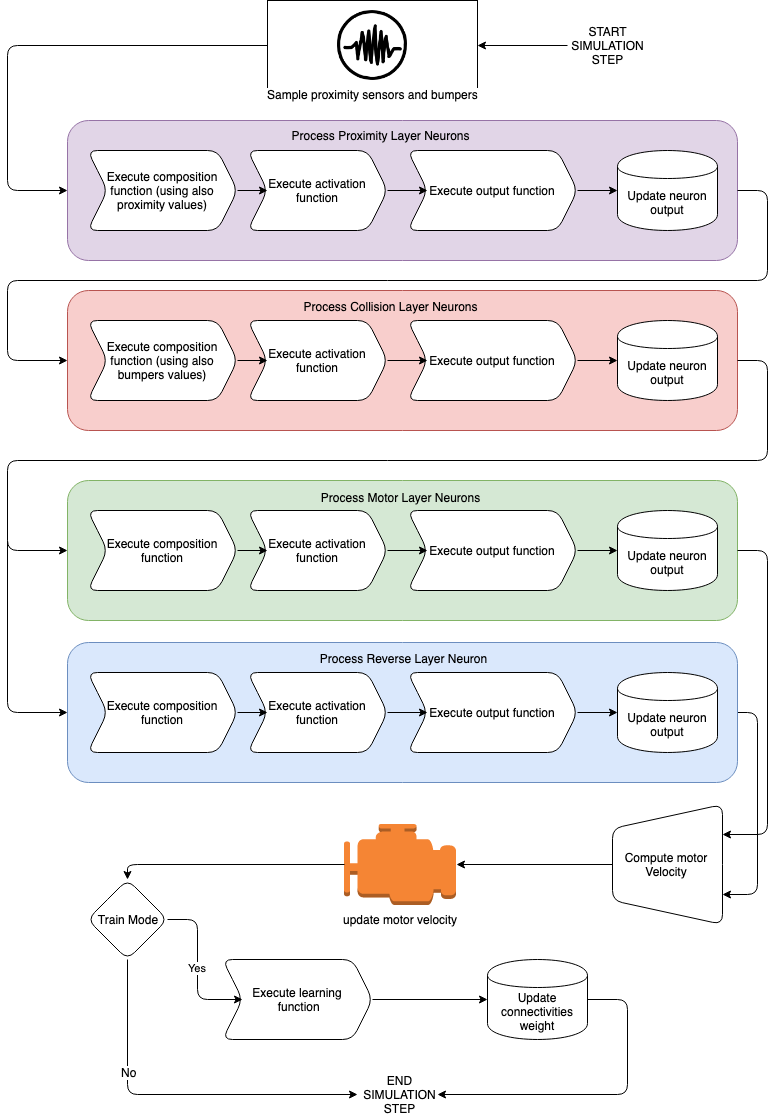
\includegraphics[scale=0.45]{figures/SimulationStep.png}
    \caption{Logica evolutiva della rete}
    \label{fig:evolutionLogic}
\end{figure}

%dettagli sull'implementazione dei riflessi dei motori
Entrando nel merito della gestione dei riflessi dei motori, come già precedentemente citato, all'interno del materiale di ricerca consultato vi erano solo indicazioni vaghe relativamente a come fossero realmente implementati. 
Perciò in questo caso abbiamo effettuato una progettazione autonoma e delle prove implementative per vedere quali fossero la strategie più adatte a gestire le nostre esigenze. Abbiamo ad esempio provato ad applicare velocità fisse, dinamiche e/o a cercare di ottenere gradi di sterzata predefiniti.
Alla fine si è deciso di prendere come valore base della velocità il valore d'uscita dei neuroni del livello motore. Ciò permette di ottenere un valore proporzionale al numero di neuroni attivi nel livello di collisione e quindi deviare maggiormente verso la direzione dove vengono rilevati meno ostacoli.

A tali velocità vengono poi applicati dei controlli:
\begin{itemize}
    \item Il primo evita che il robot rimanga fermo verificando se entrambe le velocità sono a 0. In tal caso la velocità da assegnare alle ruote viene impostata ad un valore di default predefinito.
    \item Il secondo controllo viene effettuato nel caso in cui il neurone di \textit{reverse} sia attivo. In tal caso viene controllato quale tra le due velocità è la minore e per essa viene impostato un valore negativo della velocità. Questo in caso di reverse, porterà il robot a girare su stesso verso la direzione dove vi sono meno ostacoli. Nel caso in cui le due velocità siano uguali si è scelto di sterzare sempre verso destra.
\end{itemize} 